\documentclass{article}
\usepackage{fancyhdr} % Required for custom headers
\usepackage{lastpage} % Required to determine the last page for the footer
\usepackage{extramarks} % Required for headers and footers
\usepackage{graphicx} % Required to insert images
%\usepackage{lipsum} % Used for inserting dummy 'Lorem ipsum' text into the template
\usepackage{amsmath}
%\usepackage{amsfont}
%\usepackage{amssymb}

\usepackage{multicol}
% Margins
\topmargin=-0.5in
\evensidemargin=0in
\oddsidemargin=-0.5in
\textwidth=7.5in
\textheight=9.0in
\headsep=0.25in 


\pagestyle{fancy}

\rhead{M. Adam} % Top right header
\lhead{Lemon Herb Chicken}
\chead{ }
%\title{}

\begin{document}
%
%PRELIMINARIES:
%
%
%Begin by preheating the oven to 350 $^o$F
%
%\bigskip
%
%\bigskip

\begin{multicols}{2}
Ingredients:
\begin{itemize}
\item 12 chicken drumsticks or thighs (or use a combination depending on your preference)
\item 1 bunch chives
\item 1 bunch of curly leaf parsley
\item 1/4 cup olive oil
\item 3 tbsps lemon juice (approx. yield from one lemon)
\item 2 tsps honey
\item 2 cloves of garlic
\item 1 tsp salt
\item 6-8 large basil leaves
\end{itemize}



\columnbreak

Directions:
\begin{enumerate}
\item Start by placing the chives and parsley into the food processor. Add only the top part of the parsley and not the stem. Add in olive oil, touch of lemon juice, honey and blend all of these ingredients until you have a nice paste.

\item Add in the garlic and a little bit of salt and blend. Add in the basil and blend once again.

\item Rub the herb marinade evenly on the chicken. In an oven proof pan place your chicken and cover it with plastic wrap to marinade in the refrigerator for 1-2 hours or over night.

\item Remove the plastic wrap and bake uncovered for 25 minutes in a 350°F oven until it browns. Cover the chicken with foil and place it back in the oven for 30 minutes to cook it through. To make sure your chicken is all the way cooked, cut off a piece and check.

\item Once the chicken is cooked through you are ready to serve!
\end{enumerate}
\end{multicols}



\begin{center}
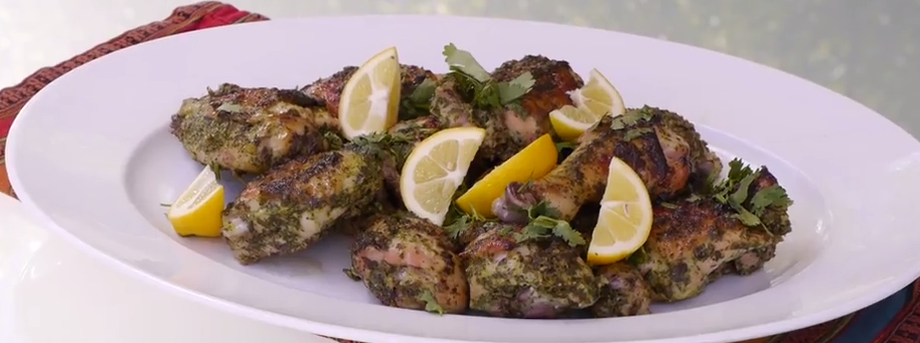
\includegraphics[scale=0.4]{LemonHerbChicken.png}
\end{center}


\end{document} 











